\documentclass[11pt]{article}

\usepackage{mathptmx}
\usepackage{url}
\usepackage{graphicx}

\newcommand*{\p}[1]{\textup{\texttt{#1}}}
\newcommand*{\ls}{\textsc{LearnSAT}}
\newcommand*{\pl}{\textsc{Prolog}}
\newcommand*{\sw}{\textsc{SWI-Prolog}}
\newcommand*{\dt}{\textsc{dot}}

\textwidth=15cm
\textheight=21cm
\topmargin=0pt
\headheight=0pt
\oddsidemargin=5mm
\headsep=0pt
\renewcommand{\baselinestretch}{1.1}
\setlength{\parskip}{0.20\baselineskip plus 1pt minus 1pt}
\parindent=0pt

\title{\bfseries \ls --- Tutorial\\\mbox{}\\\mbox{}\\
\bfseries\normalsize Version 1.1}

\author{\bfseries Mordechai (Moti) Ben-Ari\\\mbox{}\\
\url{http: //www.weizmann.ac.il/sci-tea/benari/}}

\begin{document}

\maketitle

\thispagestyle{empty}

\vspace*{\fill}

\begin{center}
\copyright{} 2012-13 by Mordechai (Moti) Ben-Ari.
\end{center}
This work is licensed under the Creative Commons Attribution-ShareAlike 3.0
License. To view a copy of this license, visit
\url{http://creativecommons.org/licenses/by-sa/3.0/}; or, (b) send a letter
to Creative Commons, 543 Howard Street, 5th Floor, San Francisco,
California, 94105, USA.

\newpage

\section{Overview}

\ls{} is a program for learning about SAT solving. It implements the
classic \emph{Davis-Putnam-Logemann-Loveland (DPLL)} algorithm, together
with modern extensions of the algorithm: \emph{conflict-driven clause
learning (CDCL)} and \emph{non-chronological backtracking (NCB)}. For a
gentle introduction to SAT solvers, see \cite[Chapter~6]{mlcs}. The
comprehensive reference is the \emph{Handbook of Satisfiability}
\cite{SAT}.

For instructions on how to run \ls{} see the User's Guide in the \ls{}
distribution.

This document is a tutorial on SAT solving with \ls{}. The algorithms
and notation follow \cite{mlm}. Some printouts have been reformatted or
edited.

\section{The DPLL algorithm}

For the tutorial, we use the set of clauses from \cite{mlm} as our
example.\footnote{\ls{} tries decision assignments in lexicographic
order, so \p{x21} and \p{x31} had a \p{0} added to their names to
preserve the order in \cite{mlm}. From Version 1.3.1 of \ls{}, the order
can be specified, so this is no longer needed.}

\begin{verbatim}
  1. [x1,x031,~x2]   2. [x1,~x3]         3. [x2,x3,x4]
  4. [~x4,~x5]       5. [x021,~x4,~x6]   6. [x5,x6]
\end{verbatim}

The file \p{examples.pro} contains the predicate \p{mlm} that runs
\p{dpll} on this set of clauses:

\begin{verbatim}
mlm :-
  dpll( [  [x1, x031, ~x2], [x1, ~x3], [x2, x3, x4],
           [~x4, ~x5], [x021, ~x4, ~x6], [x5, x6]     ], _).
\end{verbatim}

When the DPLL algorithm is run on the set of clauses, it assigns
0 to \p{x021}, \p{x031} and \p{x1}:

\begin{verbatim}
?- mlm.
LearnSAT v1.3.4. Copyright 2012-13 by Moti Ben-Ari. GNU GPL.
Decision assignment: x021=0
Decision assignment: x031=0
Decision assignment: x1=0
\end{verbatim}

Clause 1 is now a unit clause \verb+[~x2]+ implying that \p{x2} must be
assigned 0; clause 2 is also a unit clause \verb+[~x3]+ implying that
\p{x3} must be assigned 0:

\begin{verbatim}
Propagate unit: ~x2 (x2=0) derived from: 1. [x1,x031,~x2]
Propagate unit: ~x3 (x3=0) derived from: 2. [x1,~x3]
\end{verbatim}

This in turn leads to a sequence of unit propagations until clause 6
is falsified:

\begin{verbatim}
Propagate unit:  x4 (x4=1) derived from: 3. [x2,x3,x4]
Propagate unit: ~x5 (x5=0) derived from: 4. [~x4,~x5]
Propagate unit: ~x6 (x6=0) derived from: 5. [x021,~x4,~x6]
Conflict clause: 6. [x5,x6]
\end{verbatim}

Now, the algorithm backtracks, trying the assignment of 1 to \p{x1} and
then 0 to \p{x2} and \p{x3}:
\begin{verbatim}
Decision assignment: x1=1
Decision assignment: x2=0
Decision assignment: x3=0
\end{verbatim}
which causes another sequence of unit propagations leading to the same
conflict clause:
\begin{verbatim}
Propagate unit:  x4 (x4=1) derived from: 3. [x2,x3,x4]
Propagate unit: ~x5 (x5=0) derived from: 4. [~x4,~x5]
Propagate unit: ~x6 (x6=0) derived from: 5. [x021,~x4,~x6]
Conflict clause: 6. [x5,x6]
\end{verbatim}

The algorithm backtracks to assign 1 to \p{x3}, followed by 0 to \p{x4}
and \p{x5}; then, unit propagation results in assigning 1 to \p{x6}:

\begin{verbatim}
Decision assignment: x3=1
Decision assignment: x4=0
Decision assignment: x5=0
Propagate unit: x6 derived from: 6. [x5,x6]
\end{verbatim}

The result is a set of assignments that satisfies the set of clauses:

\begin{verbatim}
Satisfying assignments:
[x021=0,x031=0,x1=1,x2=0,x3=1,x4=0,x5=0,x6=1]
Statistics: clauses=6, variables=8, units=9, decisions=9, conflicts=2
\end{verbatim}

\newpage

\section{Display options}

The trace of the algorithm shown in the previous section resulted from
the following display options (that are selected by default):
\p{conflict}, \p{decision}, \p{result}, \p{sorted}, \p{unit}. The option
\p{sorted} displays the assignments as a sorted list; if the option is
cleared, the assignments will be displayed in the reverse order in which
they were made:

\begin{verbatim}
Satisfying assignments:
[x6=1,x5=0,x4=0,x3=1,x2=0,x1=1,x031=0,x021=0]
\end{verbatim}

Additional data may be obtained by using the following display options.

\begin{itemize}

\item Select \p{clause} to display the clauses and their position within
the set of clauses so that you don't have to refer back to the source
code:

\begin{verbatim}
Clauses to be checked for satisfiability:
1. [x1,x031,~x2],
2. [x1,~x3],
3. [x2,x3,x4],
4. [~x4,~x5],
5. [x021,~x4,~x6],
6. [x5,x6]
\end{verbatim}

\item Select \p{variable} to display the set of \emph{unassigned}
variables before each decision assignment and select \p{partial} to
display the set of assignments \emph{so far}:

\begin{verbatim}
Variables: [x021,x031,x1,x2,x3,x4,x5,x6]
Decision assignment: x021=0
Assignments so far:
[x021=0]
Variables: [x031,x1,x2,x3,x4,x5,x6]
Decision assignment: x031=0
Assignments so far:
[x031=0,x021=0]
Variables: [x1,x2,x3,x4,x5,x6]
Decision assignment: x1=0
Assignments so far:
[x1=0,x031=0,x021=0]
Propagate unit: ~x2 (x2=0) derived from: 1. [x1,x031,~x2]
Assignments so far:
[x2=0,x1=0,x031=0,x021=0]
\end{verbatim}

These options save the effort of frequent scrolling when tracing the
algorithm.

\item Select \p{assignment} to display the set of assignments that caused a
clause to become a conflict clause:
\begin{verbatim}
Conflict clause: 6. [x5,x6]
Conflict caused by assignments:
[x021=0,x031=0,x1=0,x2=0,x3=0,x4=1,x5=0,x6=0]
\end{verbatim}
This is an alternative to selecting \p{partial} because it just displays
the set of assignments when a conflict has been reached.

\item Select \p{evaluate} to display how each clause is evaluated when a
new assignment is tried:

\begin{verbatim}
Decision assignment: x021=0
Evaluate: [x021,~x4,~x6] has literal x021 deleted
Decision assignment: x031=0
Evaluate: [x1,x031,~x2] has literal x031 deleted
Evaluate: [x021,~x4,~x6] has literal x021 deleted
Decision assignment: x1=0
Evaluate: [x1,x031,~x2] has literal x1 deleted
Evaluate: [x1,x031,~x2] has literal x031 deleted
Evaluate: [x1,x031,~x2] is a unit clause
Evaluate: [x1,~x3] has literal x1 deleted
Evaluate: [x1,~x3] is a unit clause
Evaluate: [x021,~x4,~x6] has literal x021 deleted
Propagate unit: ~x2 (x2=0) derived from: 1. [x1,x031,~x2]
Evaluate: [x1,x031,~x2] has literal x1 deleted
Evaluate: [x1,x031,~x2] has literal x031 deleted
Evaluate: [x1,x031,~x2] is true
Evaluate: [x1,~x3] has literal x1 deleted
Evaluate: [x1,~x3] is a unit clause
\end{verbatim}
\emph{Warning}: This display option results in extremely verbose output
and would only be used in the initial stages of learning about DPLL.

\end{itemize}

\newpage

\section{Assignment trees}

Select \p{tree} to see a tree of the assignments
(Figure~\ref{tree1}).\footnote{This tree is different from the standard
semantic tree where the nodes are the variables and the edges are the
assignments. Here, the nodes are the assignments and the edges are not
labeled.} The display option \p{label} adds the antecedent clauses to
nodes that implied by unit propagation.

\begin{figure}
\begin{center}
\includegraphics[keepaspectratio=true,height=.9\textheight]{tree1}
\end{center}
\caption{Tree of assignments for the DPLL algorithm}\label{tree1}
\end{figure}

Decision assignments are in red; assignments implied by unit propagation
are in black; conflict nodes have a double red border; the node where
the satisfying assignments are found has a double green border.
You can see that the DPLL search backtracked to try assigning 1 to
\p{x1} after trying 0 and to try assigning 1 to \p{x3} after trying 0.

You can select \p{tree\_inc} to generate the trees incrementally,
whenever a conflict is reached.

%\clearpage

\section{Improving efficiency with learned clauses}

Let us run the same example with conflict-directed clause learning by setting the mode:

\begin{verbatim}
?- set_mode(cdcl).
\end{verbatim}

The display options relevant to this mode selected by default are:
\p{learned}, \p{resolvent}, \p{uip}.

After encountering the conflict clause \verb+[x5,x6]+, the algorithm
\emph{learns} the clause \verb+[x021,~x4]+ as described in
Section~\ref{learned.res}. Now, when backtracking to try the assignment
of 1 to \p{x3}, the learned clause becomes a unit clause based upon the
previous assignment of 0 to \p{x021}. Unit propagation quickly leads to
a satisfying assignment:

\begin{verbatim}
Conflict clause: 6. [x5,x6]
  . . .
Learned clause from resolution (used): [x021,~x4]
Decision assignment: x1=1@3
Propagate unit: ~x4 (x4=0@3) derived from: 7. [x021,~x4]
Decision assignment: x2=0@4
Propagate unit:  x3 (x3=1@4) derived from: 3. [x2,x3,x4]
Decision assignment: x5=0@5
Propagate unit:  x6 (x6=1@5) derived from: 6. [x5,x6]
Satisfying assignments:
[x021=0@1,x031=0@2,x1=1@3,x2=0@4,x3=1@4,x4=0@3,x5=0@5,x6=1@5]
Statistics: clauses=6, variables=8, units=8, decisions=6, conflicts=1
\end{verbatim}
Assignments are displayed together with their levels. Each decision
assignment increases the level, while assignments implied by unit
propagation receive the level of the last decision assignment. 

The search with CDCL is more efficient: compare the statistics (6
decisions and 1 conflict instead of 9 decisions and 2 conflicts) or the
the tree of assignments (Figure~\ref{tree2}).

\begin{figure}
\begin{center}
\includegraphics[keepaspectratio=true,height=.9\textheight]{tree2}
\end{center}
\caption{Tree of assignments for the DPLL algorithm with CDCL}\label{tree2}
\end{figure}

\clearpage

\section{The implication graph}

When a conflict clause is found, an \emph{implication graph} is
constructed and used to learn a clause. Select \p{graph} to display a
textual representation of an graph (first the nodes and then the edges):
\begin{verbatim}
Implication graph:
[kappa, x021=0@1, x031=0@2, x1=0@3, x2=0@3, x3=0@3, x4=1@3, x5=0@3, x6=0@3]
[
x021=0@1 --5.[x021,~x4,~x6]--> x6=0@3,
x031=0@2 --1.[x1,x031,~x2]--> x2=0@3,
x1=0@3 --1.[x1,x031,~x2]--> x2=0@3,
x1=0@3 --2.[x1,~x3]--> x3=0@3,
x2=0@3 --3.[x2,x3,x4]--> x4=1@3,
x3=0@3 --3.[x2,x3,x4]--> x4=1@3,
x4=1@3 --4.[~x4,~x5]--> x5=0@3,
x4=1@3 --5.[x021,~x4,~x6]--> x6=0@3,
x5=0@3 --6.[x5,x6]--> kappa,
x6=0@3 --6.[x5,x6]--> kappa
]
\end{verbatim}

Select \p{dot} to generate a \dt{} representation of the
graph:\footnote{Edges are labeled with the antecedent clauses because
the display option \p{label} was selected.}

\begin{center}
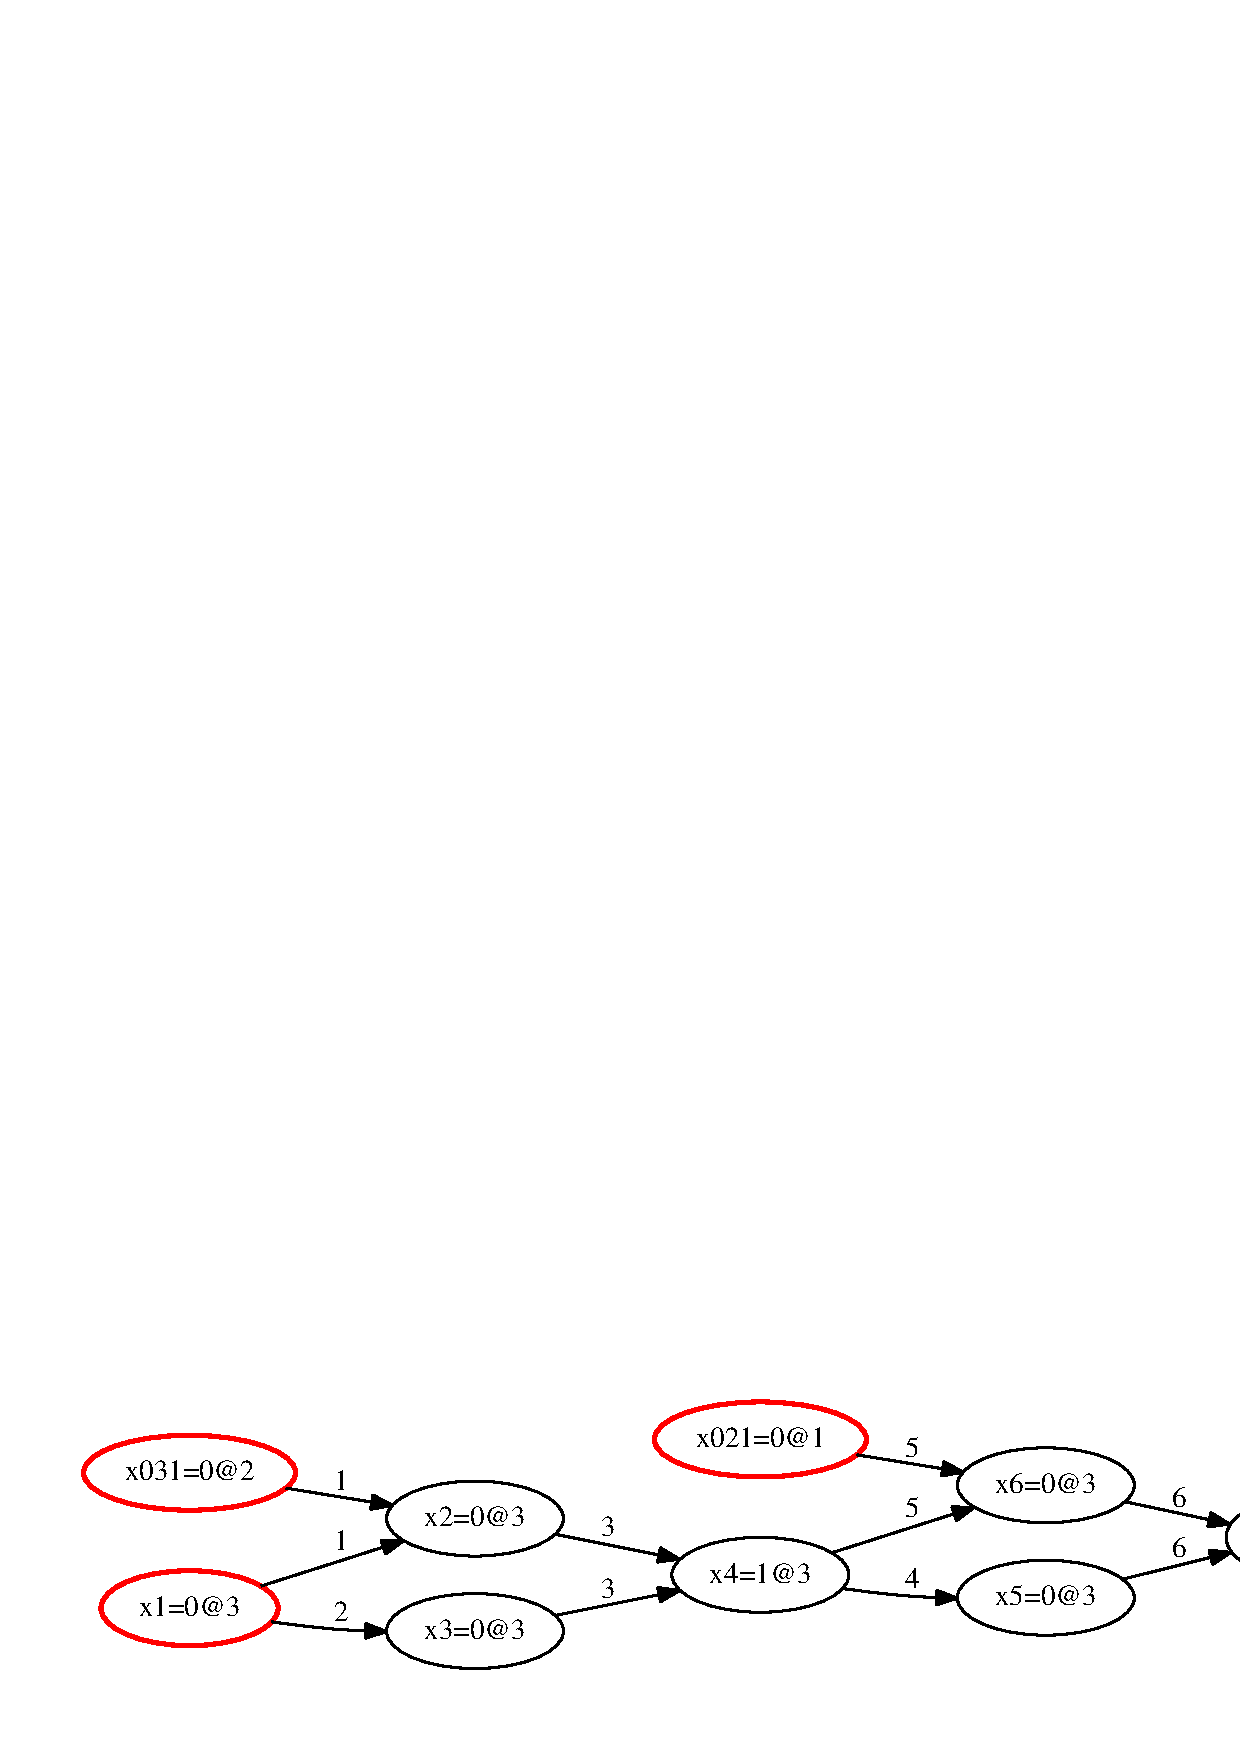
\includegraphics[keepaspectratio=true,width=\textwidth]{graph}
\end{center}

For both the textual and the \dt{} graphs, the option \p{label} was
selected to label edges with clauses and not just with their sequence
numbers.

Options \p{incremental} and \p{dot\_inc} generate the graphs after each
step of the algorithm, not just when a conflict clause is reached.

The implication graph represents the result of unit propagation that
leads to a conflict, starting from a set of decision assignments. In the
graph, are three source nodes, one for each of the decision assignments
(\p{x021=0@1}, \p{x031=0@2}, \p{x1=0@3}) that together lead to a
conflict by unit propagation.

The conflict is represented by the sink node \p{kappa} and the
assignments implied by unit propagation are represented by nodes labeled
with the assignments. An edge of the graph is labeled with the
\emph{antecedent} clause of its target node. This is the unit clause
that implied the assignment labeling that node. For example, the
decision assignments \p{x1=0@3}, \p{x031=0@2} cause \verb+[x1,x031,~x2]+
to become a unit clause and therefore this clause implies the assignment
of 0 to \p{x2}. The assignment receives the same level as the last
decision assignment so its node is labled \p{x2=0@3}.

For each non-source node, there is an incoming edge for each literal in
the unit clause except the one whose assignment is being implied.
The source nodes of these edges are labeled the assignments to those
literals. Since the clause \verb+[x1,x031,~x2]+ with three literals
implied the assignment \p{x2=0@3}, the node labeled \p{x2=0@3} has
two incoming edges: one from the node \p{x1=0@3} that assigned 0 to
\p{x1} and one from the node \p{x031@2} that assigned 0 to \p{x031},
leaving \verb+~x2+ as the unit clause that implies $x2=0@3$.

The implication graph shows that the decision assignments \p{x021=0@1},
\p{x031=0@2}, \p{x1=0@3} cause a conflict. Clearly, if
\verb+[x021,x031,x1]+ were a clause in the original set of clauses, it
would be evaluated when the decisions were made. Since it evaluates to
0, it is a conflict clause that would be found immediately and there
would be no need to carry out unit propagation. Therefore, by
\emph{learning} this clause---adding it to our original set of
clauses---any subsequent decision assignments that include these three
would immediately lead to the discovery of a conflict and shorten the
computation.

Unfortunately, there is no advantage to learning a clause based only on
these decision assignments, because the same set of decisions at levels
1, 2 and 3 will never occur again after backtracking.

Sections~\ref{learned.dom}--\ref{learned.res} present algorithms for
finding \emph{shorter} learned clauses that are more likely to become
conflict clauses as the algorithm continues. Section~\ref{learned.dom}
describes how to learn a clause by computing a dominator in the
implication graph. Section~\ref{learned.res} describes how to learn a
clause resolving backwards from the conflict node.

\emph{The two algorithms are always run one after the other.} You can
trace either one or both of the algorithms. Display option \p{dominator}
traces the computation of a dominator, and the option \p{learned}
(together with \p{resolvent}, \p{uip}, \p{literal}) traces the
computation by resolution.

\emph{Learn mode} selects which learned clause will be remembered and
subsequently used:
\begin{verbatim}
set learn_mode(dominator)    set learn_mode(resolution)
\end{verbatim}
This mode exists because the results of the two algorithms might be
different.

\newpage

\section{Learning a clause from a dominator}\label{learned.dom}

From the implication graph, we saw that a learned clause can be defined
by the decision assignments at the source nodes. However, consider all
the (four) paths from the \emph{last} decision assignment (here,
\p{x1=0@3}) to the node labeled \p{kappa} whose antecedent is the
conflict clause:\footnote{Edges are labeled with the \emph{numbers} of
the antecedent clauses because the display option \p{label} was
\emph{not} selected.}

\begin{center}
\includegraphics[keepaspectratio=true,width=\textwidth]{dom}
\end{center}

A node (here, the node labeled \p{x4=1@3}) is called a \emph{dominator}
of a decision node if it appears on all the paths from the decision node
to \p{kappa}. A dominator is a \emph{unique implication point (UIP)}
because its assignment participates in the conflict in the same way as
do \emph{all} the decision assignments that it dominates. Here, the
assignment \p{x4=1@3} is implied by the \emph{two} assignments
\p{x031=0@2} and \p{x1=0@3}, so \verb+~x4+ can replace \p{x031} and
\p{x1} in the learned clause \verb+[x021,x031,x1]+ to obtain a shorter
learned clause \verb+[x021,~x4]+.

The learned clause is therefore composed of the literal that is assigned
0 by the assignment at the UIP, together with the literals assigned at
decision assignments at \emph{lower} levels that are not dominated by
the UIP. The trace of \ls{} is:

\begin{verbatim}
Paths from the decision node at this level to kappa:
x1=0@3 --> x2=0@3 --> x4=1@3 --> x5=0@3 --> kappa
x1=0@3 --> x2=0@3 --> x4=1@3 --> x6=0@3 --> kappa
x1=0@3 --> x3=0@3 --> x4=1@3 --> x5=0@3 --> kappa
x1=0@3 --> x3=0@3 --> x4=1@3 --> x6=0@3 --> kappa
A dominator is: x4=1@3
Decisions at a lower level: [x021=0@1,x031=0@2]
Decisions not dominated: [x021=0@1]
Learned clause from dominator (not used): [x021,~x4]
\end{verbatim}

\newpage

\section{Learning a clause by resolution}\label{learned.res}

The learned clause can be obtained by resolution starting with the
conflict clause---the antecedent clause of the \p{kappa} node---and
terminating when a UIP is found. Define the conflict clause as the
initial \emph{current clause}.

At each step, the clause to be resolved with the current clause is one
that clashes with the current clause on a literal that is assigned at
the current level by unit propagation. For example, given the initial
current clause \verb+[x5,x6]+, \p{x5} was assigned by unit propagation
at this level, so we can resolve \verb+[x5,x6]+ with the antecedent
clause \verb+[~x4,~x5]+ to obtain the resolvent \verb+[~x4,x6]+ which
becomes the current clause. The next step is to resolve this clause with
\verb+[x021,~x4,~x6]+, the antecedent of the assignment to \p{x6}, to
obtain \verb+[x021,~x4]+. The resolution now terminates because clause
is associated with a UIP: there is one (implied) literal assigned at the
current level and the other literals were assigned by decision
assignments at lower levels.

The \ls{} output is:\footnote{The display option \p{literal} was
selected to display the level of the literals that are examined to find
the UIP.}

\begin{verbatim}
Conflict clause: 6. [x5,x6]
Literal: x5 assigned at level: 3
Literal: x6 assigned at level: 3
Not a UIP: two literals are assigned at level: 3
Clause: [x5,x6] unsatisfiable
Complement of: x5 assigned true in the unit clause: 4. [~x4,~x5]
Resolvent of the two clauses: [x6,~x4] also unsatisfiable
Literal: x6 assigned at level: 3
Literal: ~x4 assigned at level: 3
Not a UIP: two literals are assigned at level: 3
Clause: [x6,~x4] unsatisfiable
Complement of: x6 assigned true in the unit clause: 5. [x021,~x4,~x6]
Resolvent of the two clauses: [x021,~x4] also unsatisfiable
Literal: ~x4 assigned at level: 3
UIP: one literal is assigned at level: 3
Learned clause from resolution (used): [x021,~x4]
\end{verbatim}

Recall \cite[Theorem~4.17]{mlcs} that a resolvent $C$ is satisfiable if
and only if its parent clauses $C_1$ and $C_2$ are (simultaneously)
satisfiable. Since the conflict clause is unsatisfiable under the
current set of decision assignments, so is the set consisting of it and
its clashing clause, and therefore their resolvent---the next current
clause---is also unsatisfiable.

Let us look at the example: \verb+[x5,x6]+ is a conflict clause because
it evaluates to 0 under the assignments. The antecedent clause
\verb+[~x4,~x5]+ is a unit clause and therefore exactly one literal is
assigned 1. Since both literals in the conflict clause \verb+[x5,x6]+,
in particular \verb+x5+, are assigned 0, its complement \verb+~x5+ is
assigned 1, so it must be \emph{the single literal} in the antecedent
clause \verb+[~x4,~x5]+ that is assigned 1. Therefore, \verb+~x4+ is
assigned 0 and we can conclude that all literals in the resolvent
\verb+[~x4,x6]+ are assigned 0. In general, any resolvent generated by
resolving the conflict clause and the antecedent clauses must evaluate
to 0. We can add any of them as learned clauses without making the DPLL
algorithm incorrect.

Which of these clauses should we learn? Successive resolution steps will
eventually lead back to the clause defined by the decision nodes (here,
\verb+[x021,x031,x1]+), but, as we saw above, there is no advantage to
learning this clause. However, the resolvent clause associated with a
UIP (here, \verb+[x021,~x4]+) contains only a single literal at the
current level (here, \verb+~x4+), so it can replace the decision literal
at the same level (here, \verb+x1+), as well as any decision variables
at a lower level that are dominated by the assignment's node (here,
\verb+x031+).


\clearpage

\section{Non-chronological backtracking}

Let us now select the NCB mode:
\begin{verbatim}
?- set_mode(ncb).
\end{verbatim}

When a learned clause has been obtained, the backtrack level for
non-chronological backtracking is computed. This is the highest level of
an assignment in the learned clause except for the current level. In the
example, the learned clause is \verb+[x021,~x4]+, where \p{x4} was
assigned at level 3, the current level, and \p{x021} was assigned at
level 1 which becomes the backtrack level. When backtracking, we can
skip decision assignments whose level is at a lower level than the
backtrack level, in the example, the decision assignments at levels 3
and 2:

\begin{verbatim}
Non-chronological backtracking to level: 1
Skip decision assignment: x1=1@3
Skip decision assignment: x031=1@2
\end{verbatim}

NCB can be seen in the tree of assignments (Figure~\ref{tree3}). The
graph is no longer a tree but a DAG (directed acyclic graph) because
once \p{x021} is assigned (0 or 1), the assignments of 0 to \p{x031} and
then \p{x1} lead to the same sequence of unit propagations. The graph
branches only at its leaves because one assignment leads to a conflict
clause and the other to a satisfying assignment.

\begin{figure}
\begin{center}
\includegraphics[keepaspectratio=true,height=.9\textheight]{tree3}
\end{center}
\caption{Tree of assignments for the DPLL algorithm with CDCL and NCB}\label{tree3}
\end{figure}


\newpage

\bibliographystyle{plain}
\bibliography{learnsat}
\end{document}
